\documentclass[10.5pt,a4paper]{article}
\usepackage[utf8]{inputenc}
\usepackage[T1]{fontenc}
\usepackage{amsmath,amssymb}
\usepackage{geometry}
\geometry{margin=1.8cm}
\usepackage{tikz}
\usetikzlibrary{arrows.meta}
\usepackage{xcolor}
\usepackage{enumitem}

\definecolor{ans}{RGB}{20,90,50}
\definecolor{cbleu}{RGB}{30,90,200}
\definecolor{cvert}{RGB}{20,140,60}
\definecolor{corange}{RGB}{225,130,15}
\definecolor{crouge}{RGB}{200,30,30}

\newcounter{q}
\newcommand{\qa}[2]{%
  \refstepcounter{q}%
  \par\noindent\textbf{\theq.} #1\\
  \textcolor{ans}{\textbf{$\rightarrow$ #2}}\par\vspace{5pt}%
}

\title{\textbf{Questions préliminaires -- Réponses courtes}\\[2pt]\large Mécanique et thermodynamique}
\author{}
\date{}

\begin{document}
\maketitle
\vspace{-0.9cm}
\begin{center}
\small\itshape Réponses volontairement courtes (format flashcard) -- une bonne réponse d'examen peut être
aussi brève que celles-ci.
\end{center}
\vspace{0.3cm}

\setlength{\parskip}{0pt}

\qa{Quelle est l'unité SI d'une énergie ?}{Joule (J)}
\qa{Quelle est l'unité SI d'une puissance ?}{Watt (W)}
\qa{Quelle est l'unité SI d'une pression ?}{Pascal (Pa)}
\qa{Quelle est l'unité SI d'un volume ?}{m$^3$}
\qa{Quelle est l'unité SI d'une température ?}{Kelvin (K)}
\qa{Quel est le lien entre 1 Joule et 1 Watt ?}{1 W = 1 J/s}
\qa{Quel est le signe d'une énergie entrant dans le système ?}{Positif}
\qa{Quel est le signe d'une énergie sortant du système ?}{Négatif}
\qa{Donnez la formule de la loi des gaz parfaits}{$pV=nRT$}
\qa{Que vaut $R$, la constante des gaz parfaits (valeur et unité) ?}{$R=8{,}314$ J/(mol$\cdot$K)}
\qa{Quelle est la caractéristique d'une courbe isobare ?}{$p=$ constante}
\qa{Quelle est la caractéristique d'une courbe isochore ?}{$V=$ constante}
\qa{Quelle est la caractéristique d'une isotherme ?}{$T=$ constante (donc $pV=$ constante pour un gaz parfait)}
\qa{Quelle est la caractéristique d'une adiabatique réversible ?}{$Q=0$, on peut revenir à l'état initial
(isentropique, $S=$ constante)}
\qa{Quelle est la formule générale du travail élémentaire réversible ?}{$W=-\displaystyle\int_{V_i}^{V_f}p\,dV$}

\par\noindent\textbf{\stepcounter{q}\theq.} Sur le graphe suivant, le travail est-il positif, négatif ou nul ?
\begin{center}
\begin{tikzpicture}[scale=0.75, >=Stealth]
\draw[->] (0,0) -- (5.5,0) node[right] {$V$};
\draw[->] (0,0) -- (0,4) node[above] {$p$};
\draw[thick,->] (1,0.8) to[out=70,in=180] (2.3,2.1) to[out=0,in=160] (4.5,3.2);
\fill (1,0.8) circle (1.6pt) node[below left]{$i$};
\fill (4.5,3.2) circle (1.6pt) node[above right]{$f$};
\end{tikzpicture}
\end{center}
\textcolor{ans}{\textbf{$\rightarrow$ Négatif} ($V$ augmente globalement de $i$ à $f$ : c'est une détente,
le système fournit du travail à l'extérieur $\Rightarrow W<0$.)}
\vspace{5pt}

\par\noindent\textbf{\stepcounter{q}\theq.} Sur le graphe suivant, le cycle est-il récepteur ou moteur ?
\begin{center}
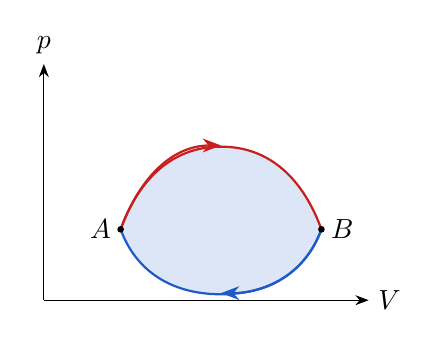
\begin{tikzpicture}[scale=0.75, >=Stealth]
\draw[->] (0,0) -- (5.5,0) node[right] {$V$};
\draw[->] (0,0) -- (0,4) node[above] {$p$};
\fill[cbleu!15] (1.3,1.2) to[out=70,in=180] (3,2.6) to[out=0,in=110] (4.7,1.2)
  to[out=250,in=0] (3,0.1) to[out=180,in=290] (1.3,1.2);
\draw[thick,crouge] (1.3,1.2) to[out=70,in=180] (3,2.6) to[out=0,in=110] (4.7,1.2);
\draw[thick,crouge,->] (1.3,1.2) to[out=70,in=180] (3,2.62);
\draw[thick,cbleu] (4.7,1.2) to[out=250,in=0] (3,0.1) to[out=180,in=290] (1.3,1.2);
\draw[thick,cbleu,->] (4.7,1.2) to[out=250,in=0] (3,0.12);
\fill (1.3,1.2) circle (1.6pt) node[left]{$A$};
\fill (4.7,1.2) circle (1.6pt) node[right]{$B$};
\end{tikzpicture}
\end{center}
\textcolor{ans}{\textbf{$\rightarrow$ Moteur} (sens horaire : \textcolor{crouge}{détente en haut, haute
pression} puis \textcolor{cbleu}{compression en bas, basse pression} $\Rightarrow$ travail net fourni,
$W_{tot}<0$ ; l'aire du cycle = $|W_{tot}|$.)}
\vspace{5pt}

\qa{Quelle est la formule générale du premier principe de la thermo ?}{$\Delta U=W+Q$}
\qa{Quelle est la formule du premier principe pour un cycle fermé ?}{$W+Q=0$}
\qa{Quelle est l'unité d'une chaleur spécifique molaire ?}{J/(mol$\cdot$K)}
\qa{Pour quel type de transformation puis-je utiliser $T V^{\gamma-1}{=}$const, $pV^\gamma{=}$const et
$T^\gamma V^{1-\gamma}{=}$const ?}{Une transformation adiabatique réversible (gaz parfait)}

\par\noindent\textbf{\stepcounter{q}\theq.} Tracez dans un diagramme $p$-$V$ la forme d'une adiabatique,
d'une isotherme, d'une isobare et d'une isochore passant par un même point.
\begin{center}
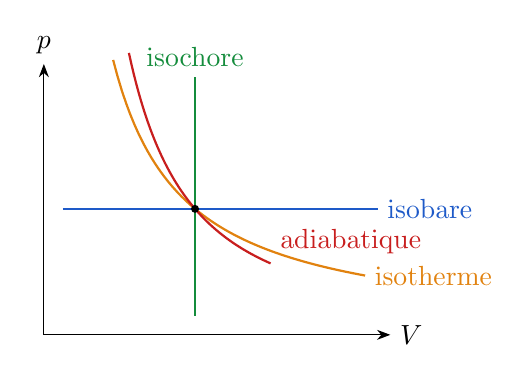
\begin{tikzpicture}[scale=0.8, >=Stealth]
\draw[->] (0,0) -- (5.5,0) node[right] {$V$};
\draw[->] (0,0) -- (0,4.3) node[above] {$p$};
\coordinate (P) at (2.4,2);
\draw[thick,cvert] (2.4,0.3) -- (2.4,4.1); \node[cvert,above] at (2.4,4.1) {isochore};
\draw[thick,cbleu] (0.3,2) -- (5.3,2); \node[cbleu,right] at (5.3,2) {isobare};
\draw[thick,corange,domain=1.1:5.1,samples=60,variable=\x] plot ({\x},{2.4*2/\x});
\node[corange,right] at (5.1,{2.4*2/5.1}) {isotherme};
\draw[thick,crouge,domain=1.35:3.6,samples=60,variable=\x] plot ({\x},{2.4^1.4*2/(\x^1.4)});
\node[crouge,above right] at (3.6,{2.4^1.4*2/(3.6^1.4)}) {adiabatique};
\fill (P) circle (1.8pt);
\end{tikzpicture}
\end{center}
\textcolor{ans}{\textbf{$\rightarrow$} \textcolor{cvert}{Isochore = verticale}, \textcolor{cbleu}{isobare =
horizontale}, \textcolor{corange}{isotherme = hyperbole ($pV{=}$cste)}, \textcolor{crouge}{adiabatique =
hyperbole plus pentue que l'isotherme ($pV^\gamma{=}$cste, $\gamma>1$)}.}
\vspace{5pt}

\qa{Machine MOTRICE : signes de $Q_1$ (source chaude), $Q_2$ (source froide), $W$ (total) ?}{$Q_1>0$,
$Q_2<0$, $W<0$}
\qa{Quelle est la formule générale du rendement d'un cycle moteur ?}{$\eta=\dfrac{|W|}{Q_1}=\dfrac{\text{énergie
utile}}{\text{énergie fournie}}$}
\qa{Quelle information nous donne le rendement de Carnot d'un cycle ?}{Le rendement \textbf{maximal
théorique} (limite indépassable) entre deux sources de température données}
\qa{Quel type de transformation est utilisé pour un compresseur dans un cycle ?}{Adiabatique réversible
(isentropique)}
\qa{Quel type de transformation est utilisé pour une turbine dans un cycle ?}{Adiabatique réversible
(isentropique)}
\qa{Quel type de transformation est utilisé pour un échangeur dans un cycle ?}{Isobare}

\par\noindent\textbf{\stepcounter{q}\theq.} Quel est le schéma d'un cycle moteur essence 4 temps ?
\begin{center}
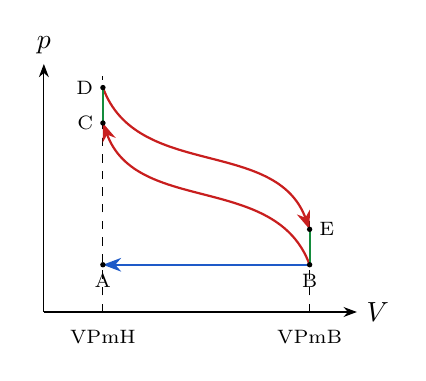
\begin{tikzpicture}[scale=0.75, >=Stealth]
\draw[->] (0,0) -- (5.3,0) node[right] {$V$};
\draw[->] (0,0) -- (0,4.2) node[above] {$p$};
\coordinate (A) at (1,0.8); \coordinate (B) at (4.5,0.8);
\coordinate (C) at (1,3.2); \coordinate (D) at (1,3.8);
\coordinate (E) at (4.5,1.4);
\draw[dashed] (1,0) -- (1,4.0); \node[below] at (1,-0.15) {\scriptsize VPmH};
\draw[dashed] (4.5,0) -- (4.5,1.7); \node[below] at (4.5,-0.15) {\scriptsize VPmB};
\draw[thick,crouge,->] (B) to[out=110,in=-70] (C);
\draw[thick,crouge,->] (D) to[out=-70,in=110] (E);
\draw[thick,cvert] (C) -- (D);
\draw[thick,cvert] (E) -- (B);
\draw[thick,cbleu,->] (B) -- (A);
\foreach \p/\lab/\pos in {A/A/below,B/B/below,C/C/left,D/D/left,E/E/right}
  {\fill (\p) circle (1.3pt) node[\pos] {\scriptsize\lab};}
\end{tikzpicture}
\end{center}
\textcolor{ans}{\textbf{$\rightarrow$} \textcolor{cbleu}{Admission (isobare, B$\to$A)} --
\textcolor{crouge}{compression (adiabatique, B$\to$C)} -- \textcolor{cvert}{explosion (isochore, C$\to$D)}
-- \textcolor{crouge}{détente (adiabatique, D$\to$E)} -- \textcolor{cvert}{échappement (isochore,
E$\to$B)}.}
\vspace{5pt}

\par\noindent\textbf{\stepcounter{q}\theq.} Quel est le schéma d'un cycle moteur diesel 4 temps ?
\begin{center}
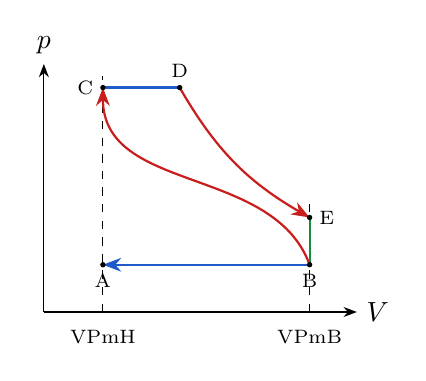
\begin{tikzpicture}[scale=0.75, >=Stealth]
\draw[->] (0,0) -- (5.3,0) node[right] {$V$};
\draw[->] (0,0) -- (0,4.2) node[above] {$p$};
\coordinate (A) at (1,0.8); \coordinate (B) at (4.5,0.8);
\coordinate (C) at (1,3.8); \coordinate (D) at (2.3,3.8);
\coordinate (E) at (4.5,1.6);
\draw[dashed] (1,0) -- (1,4.0); \node[below] at (1,-0.15) {\scriptsize VPmH};
\draw[dashed] (4.5,0) -- (4.5,1.9); \node[below] at (4.5,-0.15) {\scriptsize VPmB};
\draw[thick,crouge,->] (B) to[out=110,in=-90] (C);
\draw[thick,crouge,->] (D) to[out=-60,in=150] (E);
\draw[thick,cbleu] (C) -- (D);
\draw[thick,cvert] (E) -- (B);
\draw[thick,cbleu,->] (B) -- (A);
\foreach \p/\lab/\pos in {A/A/below,B/B/below,C/C/left,D/D/above,E/E/right}
  {\fill (\p) circle (1.3pt) node[\pos] {\scriptsize\lab};}
\end{tikzpicture}
\end{center}
\textcolor{ans}{\textbf{$\rightarrow$} \textcolor{cbleu}{Admission d'air seul (isobare, B$\to$A)} --
\textcolor{crouge}{compression (adiabatique, B$\to$C)} -- \textcolor{cbleu}{injection + combustion
(isobare, C$\to$D, pas isochore)} -- \textcolor{crouge}{détente (adiabatique, D$\to$E)} --
\textcolor{cvert}{échappement (isochore, E$\to$B)}.}
\vspace{5pt}

\qa{Comment appelle-t-on le volume dans le cylindre quand le piston est le plus haut ?}{Point mort haut
(PMH) -- volume minimal}
\qa{Comment appelle-t-on le volume dans le cylindre quand le piston est le plus bas ?}{Point mort bas
(PMB) -- volume maximal}
\qa{Quelle est la formule générale de combustion d'un hydrocarbure ?}{$C_xH_y+\left(x+\dfrac{y}{4}\right)O_2
\to xCO_2+\dfrac{y}{2}H_2O$}

\par\noindent\textbf{\stepcounter{q}\theq.} Schématisez les éléments constituant une machine frigo/PAC.
\begin{center}
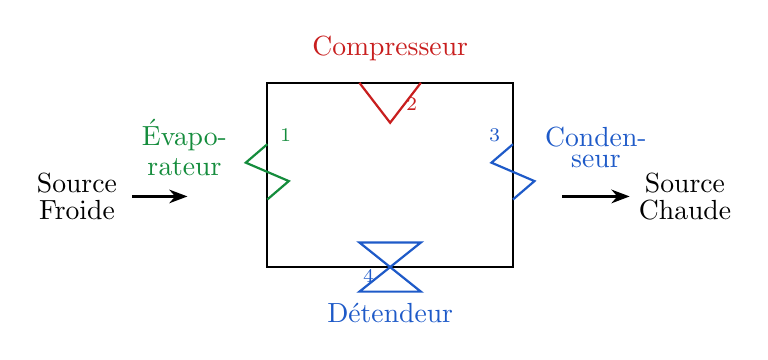
\begin{tikzpicture}[scale=0.78, >=Stealth, thick]
% boucle
\draw (0,0) -- (0,3) -- (4,3) -- (4,0) -- cycle;
% évaporateur (zigzag gauche)
\draw[cvert] (0,1.1) -- (0.35,1.4) -- (-0.35,1.7) -- (0,2.0);
\node[cvert] at (-1.35,1.95) {\shortstack{Évapo-\\rateur}};
% condenseur (zigzag droite)
\draw[cbleu] (4,1.1) -- (4.35,1.4) -- (3.65,1.7) -- (4,2.0);
\node[cbleu] at (5.35,1.95) {\shortstack{Conden-\\seur}};
% compresseur (chevron sur le haut)
\draw[crouge] (1.5,3) -- (2,2.35) -- (2.5,3);
\node[crouge] at (2,3.55) {Compresseur};
% détendeur (noeud papillon sur le bas)
\draw[cbleu] (1.5,0.4) -- (2.5,0.4) -- (2,0) -- cycle;
\draw[cbleu] (1.5,-0.4) -- (2.5,-0.4) -- (2,0) -- cycle;
\node[cbleu] at (2,-0.75) {Détendeur};
% sources
\node at (-3.1,1.15) {\shortstack{Source\\Froide}};
\draw[->] (-2.2,1.15) -- (-1.3,1.15);
\node at (6.8,1.15) {\shortstack{Source\\Chaude}};
\draw[->] (4.8,1.15) -- (5.9,1.15);
% points 1-2-3-4
\node[cvert] at (0.3,2.15) {\scriptsize 1};
\node[crouge] at (2.35,2.65) {\scriptsize 2};
\node[cbleu] at (3.7,2.15) {\scriptsize 3};
\node[cbleu] at (1.65,-0.15) {\scriptsize 4};
\end{tikzpicture}
\end{center}
\textcolor{ans}{\textbf{$\rightarrow$} \textcolor{cvert}{Évaporateur (BP, source froide)} $\to$
\textcolor{crouge}{compresseur} $\to$ \textcolor{cbleu}{condenseur (HP, source chaude)} $\to$
\textcolor{cbleu}{détendeur} $\to$ retour évaporateur -- boucle fermée par le fluide frigorigène.}

\end{document}
